\chapter{Comparing Algorithms}


% it 1
With the {\tt norMmix} package explained, we can turn to comparing it to 
existing methods. As previously stated, the implementation representing the 
EM-algorithm is the {\tt mclust} package. It will be used with very little 
deviation from out-of-the-box, safe for restriction of the covariance models.
This is done, so we can compare like with like.
The specific command that performs the EM-algorithm is:

\begin{Schunk}
\begin{Sinput}
>     #mclust::Mclust(x, G=cl, modelNames=mo)$BIC
\end{Sinput}
\end{Schunk}

Where {\tt cl} is a vector of integers of however many components we are trying 
to fit and {\tt mo} are the model names:

\begin{Schunk}
\begin{Soutput}
 [1] "EII" "VII" "EEI" "VEI" "EVI" "VVI" "EEE" "VEE" "EVV" "VVV"
\end{Soutput}
\end{Schunk}

The {\tt \$BIC} element of the results is taken as the main tool for model 
selection, as it is advertised in the package authors paper \cite{Scr16}.

There is however a small but crucial change applied to these results.
The {\tt mclust} package authors have flipped the definition of the BIC to mean:
\[ 2 ln(\hat{L}) - ln(n) \theta\]
instead of the more common
\[ ln(n) \theta - 2 ln(\hat{L}) \]
Where $n$ is the number of observations, $\theta$ is the cardinality of the 
parameter vector and $\hat{L}$ is the estimated log-likelihood.

So even if not explicitly mentioned, we use the negative of the values returned
by {\tt mclust}.

Another thing that should be stated before all else is the difference in 
initialization between {mclust}'s pre-clustering and CLARA. CLARA is dependent
on random number generators (RNG). As such, unless a fixed seed is chosen, 
every iteration of CLARA will return a different result. Unlike {\tt mclust}, 
which will, for given data, always return the same results. The effect on the 
following findings is that results will spread out for data obtained from 
CLARA results.


% it 1
First, we illustrate the structure of the graphical results we will be 
presenting hereafter. The basic shape of the plots will be the BIC value 
plotted against the number of components. This is in line with {\tt mclust}'s
manner of visualizing data, however since our method is to some extent RNG 
dependent, we are forced to display multiple runs of the algorithm on the same
graph. Therefore we split the plot according to covariance model, putting 10
models in 10 graphs in a plot. Here an example:


\begin{figure}
    \centering
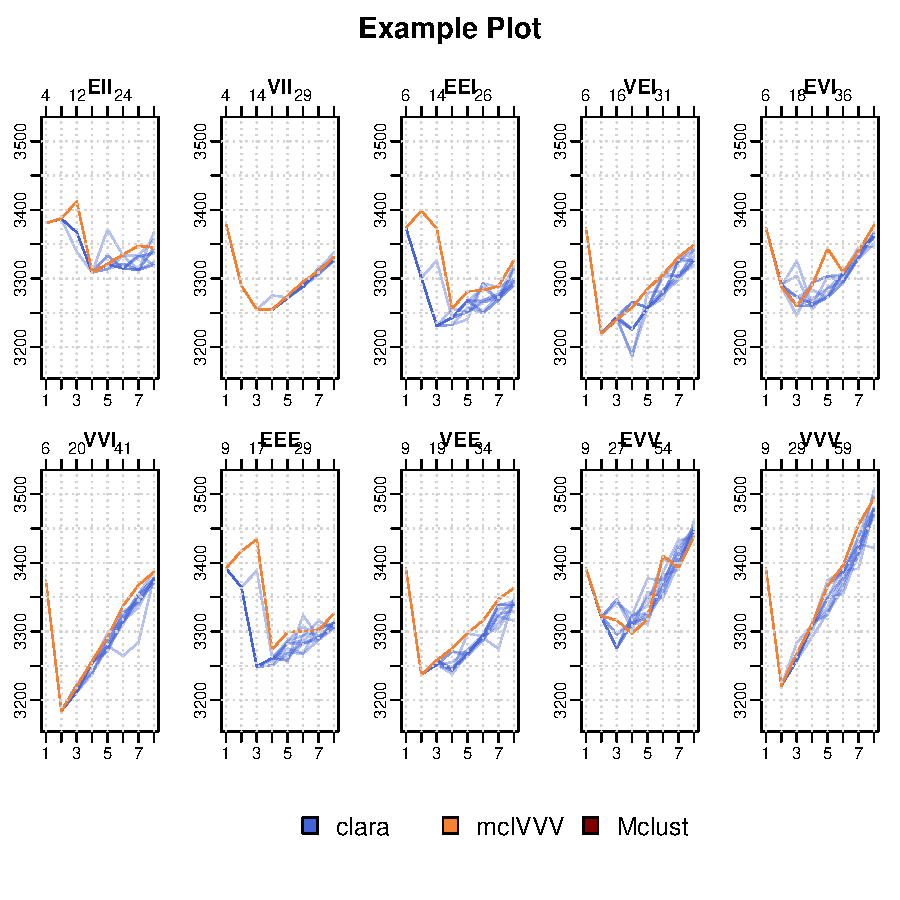
\includegraphics{chapter3-bicplotdemoplot}
    \caption{Example of Comparison Plot}
    \label{fig:ExPlot}
\end{figure}

As can be seen from the formula of the BIC value, lower is better. When 
selecting a model based on BIC, we take the model and component with the 
lowest value to be the best fitting model. Although this may not necessarily
the 'correct' model, that is, the model from which the data arises.

There are many ways in which this type of model selection might miss the 
correct model, for example by 'gluing together' multiple components into one,
or covering the dataset in a 'patchwork' of smaller components, to name a few.

We will discuss them as they arise in the following analysis of simulations

here explain simulations conducted, \ref{App:sims}
here explain the various sections: time, n, p, difficult , nonnormal 

\section{Time Analysis}

here how much time they take, in p,k and n give approximate O(x) value

\begin{Schunk}
\begin{Sinput}
>     library(norMmix, lib.loc="~/ethz/BA/norMmix.Rcheck/")
>     # change this dir to whereever the simulations are saved
>     mainsav <- normalizePath("~/ethz/BA/Rscripts/")
>     savdir <- file.path(mainsav, "2time")
>     filelist <- list.files(savdir, pattern=".rds")
>     filelist <- grep("mcl.rds", filelist, invert=TRUE, value=TRUE)
>     ## need to split these better
>     f <- lapply(file.path(savdir,filelist), function(j) readRDS(j)$fit)
>     times <- unlist(lapply(f, function(j) extracttimes(j)[,,1]))
>     dims <- unlist(lapply(f, function(j) attr(extracttimes(j), "p")))
>     size <- unlist(lapply(f, function(j) attr(extracttimes(j), "n")))
>     ddims <- rep(dims, each=80)
>     ssize <- rep(size, each=80)
>     pars <- unlist(lapply(f, npar))
>     r <- lm(log(times) ~ log(pars) + log(ddims) + log(ssize))
>     summary(r)
\end{Sinput}
\begin{Soutput}
Call:
lm(formula = log(times) ~ log(pars) + log(ddims) + log(ssize))

Residuals:
    Min      1Q  Median      3Q     Max 
-3.4428 -0.2986  0.0671  0.4579  2.0936 

Coefficients:
            Estimate Std. Error t value Pr(>|t|)    
(Intercept) -9.74133    0.10598  -91.91   <2e-16 ***
log(pars)    2.75983    0.01181  233.75   <2e-16 ***
log(ddims)  -2.06063    0.02483  -82.99   <2e-16 ***
log(ssize)   0.61301    0.01446   42.38   <2e-16 ***
---
Signif. codes:  0 ‘***’ 0.001 ‘**’ 0.01 ‘*’ 0.05 ‘.’ 0.1 ‘ ’ 1

Residual standard error: 0.6946 on 7196 degrees of freedom
Multiple R-squared:  0.8887,	Adjusted R-squared:  0.8887 
F-statistic: 1.916e+04 on 3 and 7196 DF,  p-value: < 2.2e-16
\end{Soutput}
\end{Schunk}

\begin{figure}[h]
    \centering
\begin{Schunk}
\begin{Sinput}
>     plot(times~pars, log="xy", yaxt="n", xaxt="n")
>     sfsmisc::eaxis(1)
>     sfsmisc::eaxis(2)
\end{Sinput}
\end{Schunk}
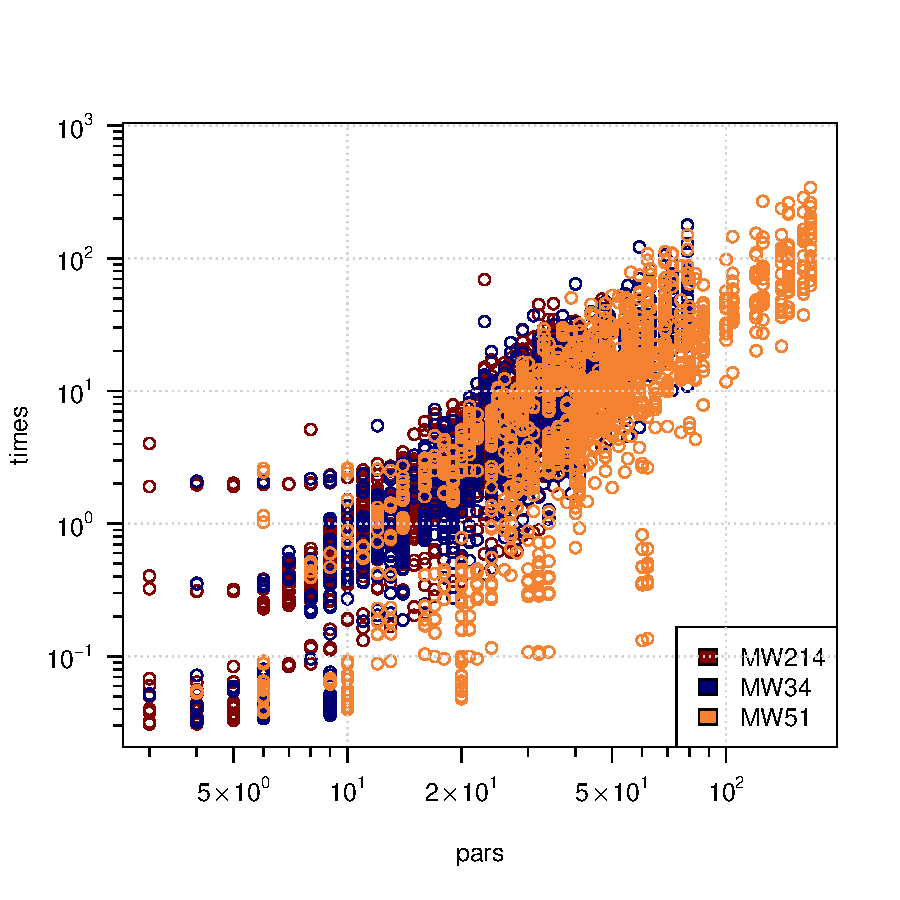
\includegraphics{chapter3-figtime}
    \caption{Log-log Plot of System Time against Parameter Length}
    \label{fig:time}
\end{figure}

can see that time is almost one to one proportional to parameter length.

\section{Behaviour in {\tt n}}

% it 1
here show as expected narrower scattering as n increases


\begin{figure}[h]
    \centering
\begin{Schunk}
\begin{Sinput}
>     compplot(s05mw34bic, m0534)
\end{Sinput}
\end{Schunk}
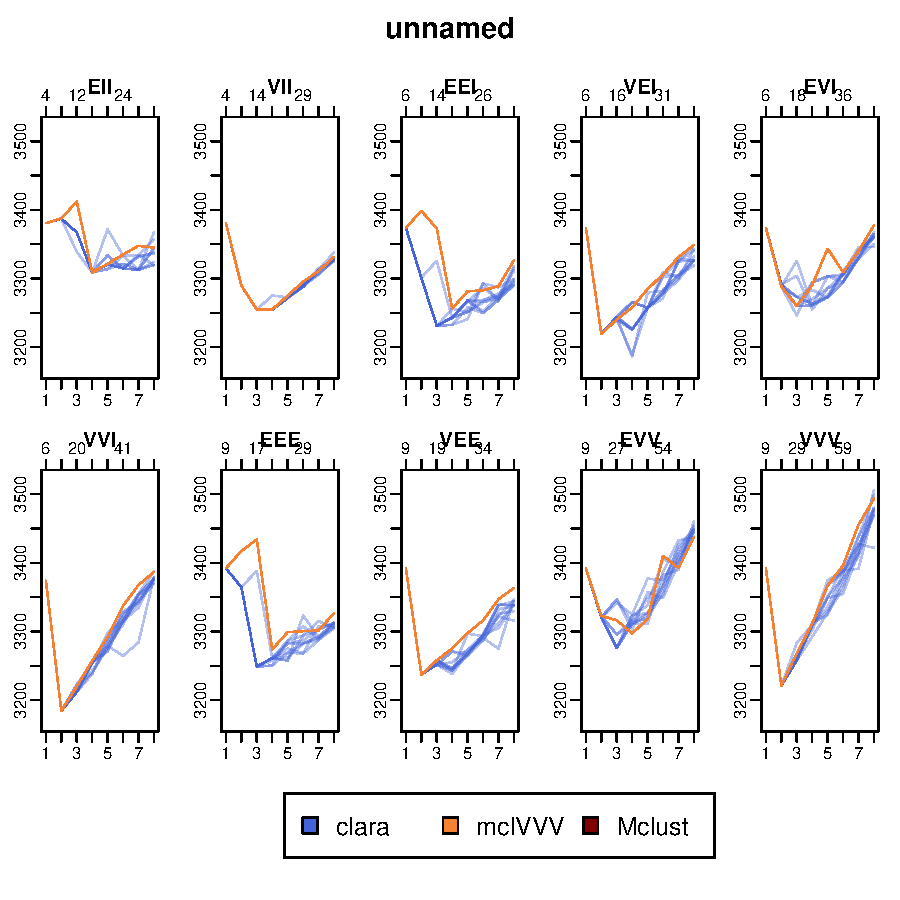
\includegraphics{chapter3-fig5fit}
\end{figure}[h]
\begin{figure}
\begin{Schunk}
\begin{Sinput}
>     compplot(s10mw34bic, m1034)
\end{Sinput}
\end{Schunk}
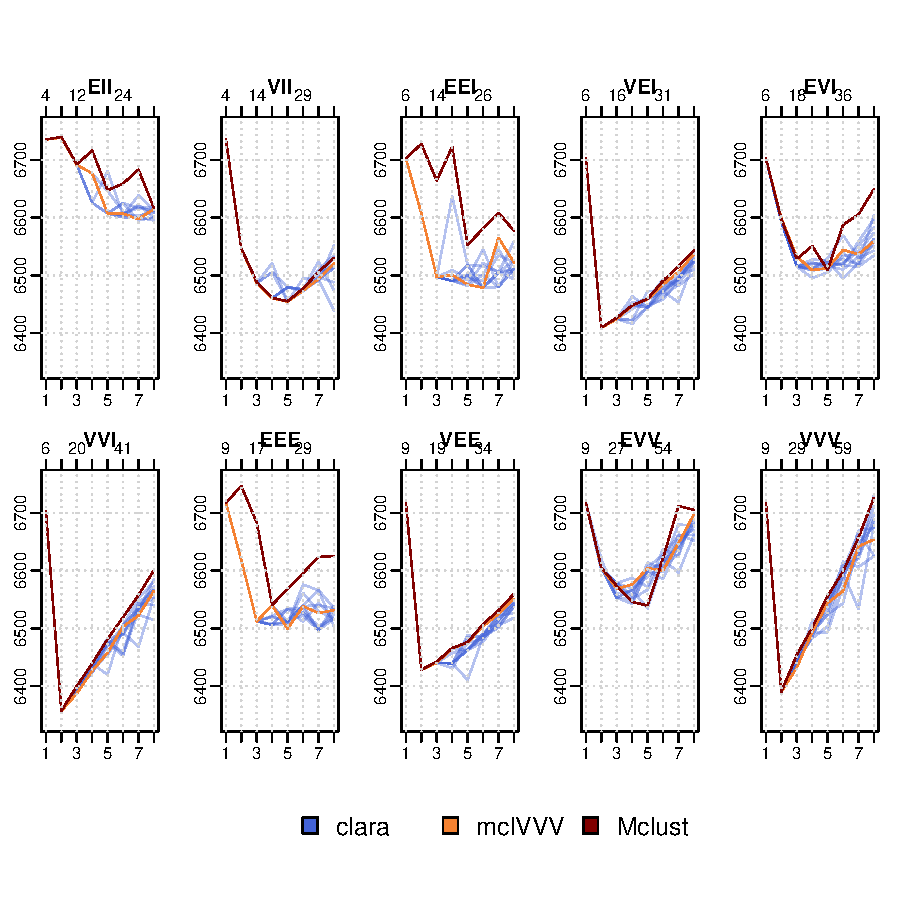
\includegraphics{chapter3-fig10fit}
\end{figure}


\section{Behaviour in {\tt p}}

% it 1
here show how norMmix is consistently competitive with mclust

\begin{figure}[h]
\begin{Schunk}
\begin{Sinput}
>     plot(MW34)
\end{Sinput}
\end{Schunk}
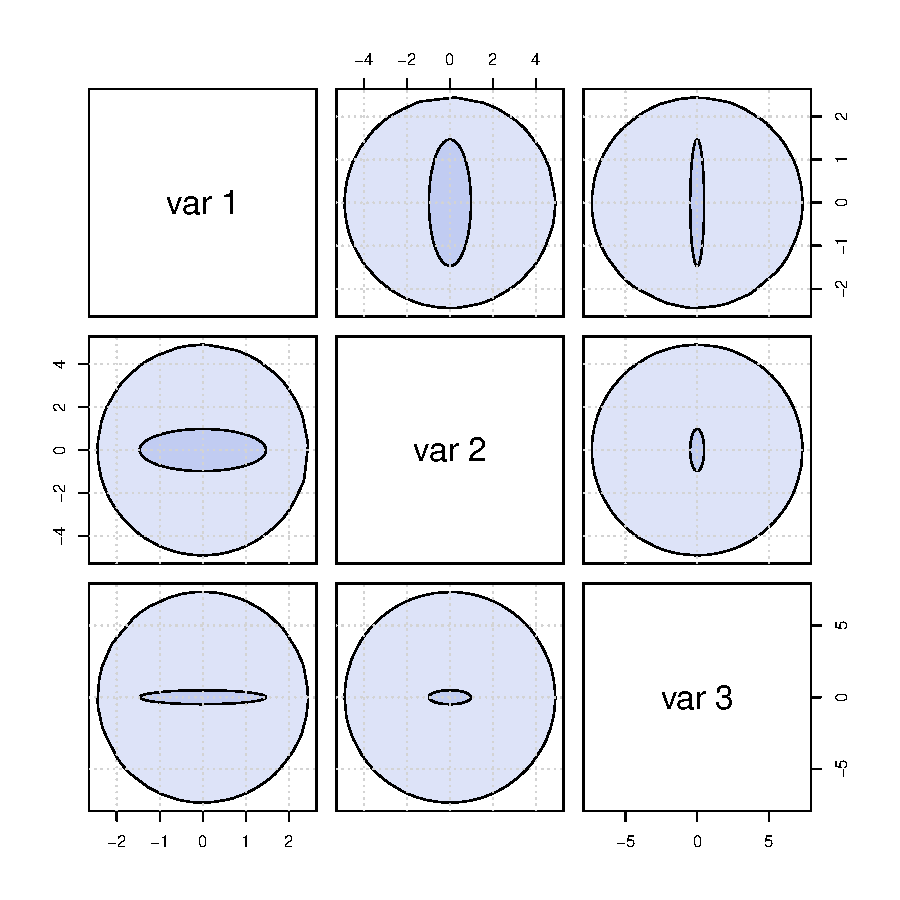
\includegraphics{chapter3-figMW34}
\end{figure}



\begin{figure}[h]
\begin{Schunk}
\begin{Sinput}
>     compplot(clarabic, mclbic, mclustbic, main="Fit of MW34")
\end{Sinput}
\end{Schunk}
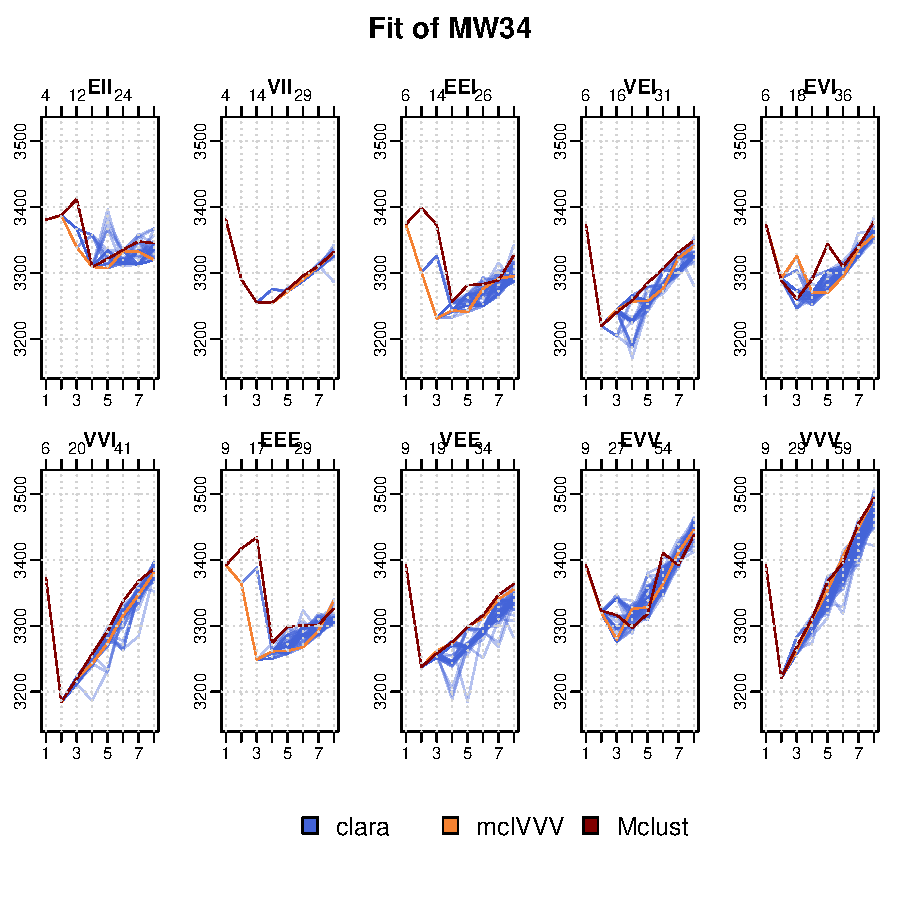
\includegraphics{chapter3-figMW34bic}
\end{figure}

\section{Diffixult Mixtures}

% it 1
here show behaviour in difficult cases

\begin{figure}[h]
\begin{Schunk}
\begin{Sinput}
>     plot(MW214)
\end{Sinput}
\end{Schunk}
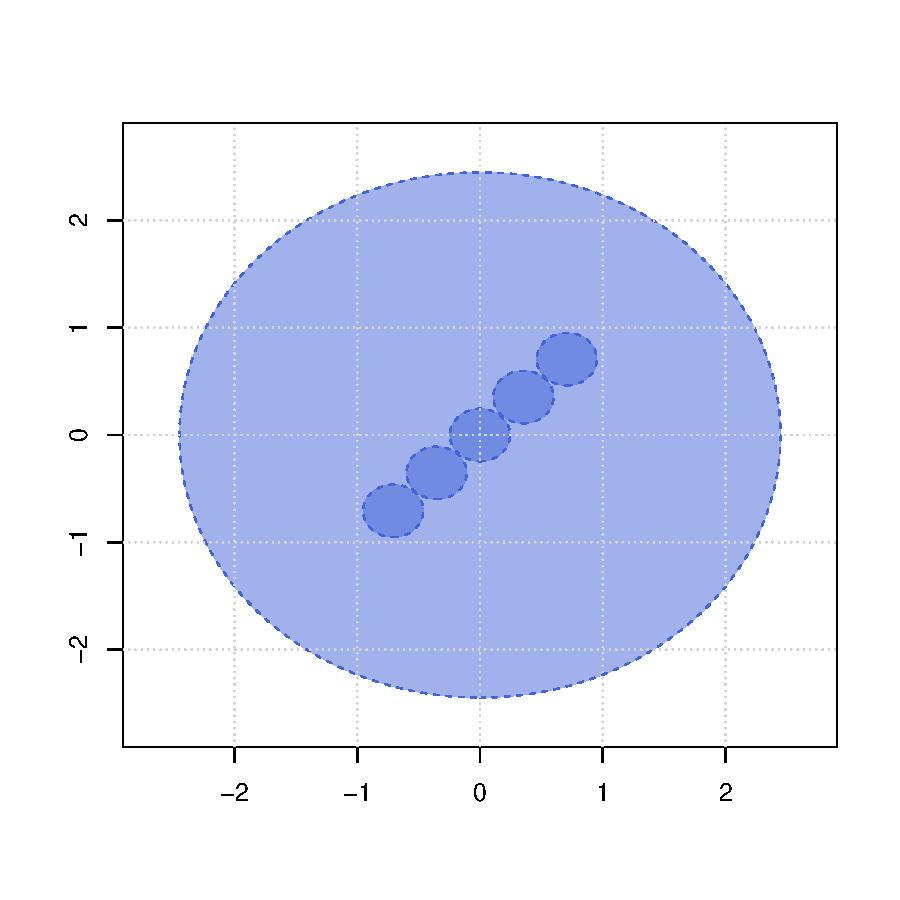
\includegraphics{chapter3-figMW214}
\end{figure}


\begin{Schunk}
\begin{Sinput}
>     savdir <- file.path(mainsav, "2init")
>     filenames <- list.files(savdir, pattern=".rds")
>     MW214fn <- grep("MW214", filenames, value="TRUE")
>     mclustfiles <- grep("mcl.rds", MW214fn, value=TRUE)
>     MW214fn <- grep("mcl.rds", MW214fn, value="TRUE", invert=TRUE)
>     claraMW <- grep("clara", MW214fn, value=TRUE)
>     mclMW <- grep("mclVVV", MW214fn, value=TRUE)
>     clarabic <- massbic(claraMW, savdir)
>     mclbic <- massbic(mclMW, savdir)
>     mclustbic <- readRDS(file.path(savdir,mclustfiles[1]))
\end{Sinput}
\end{Schunk}

\begin{figure}[h]
\begin{Schunk}
\begin{Sinput}
>     compplot(clarabic, mclbic, mclustbic, main="Fit of MW214")
\end{Sinput}
\end{Schunk}
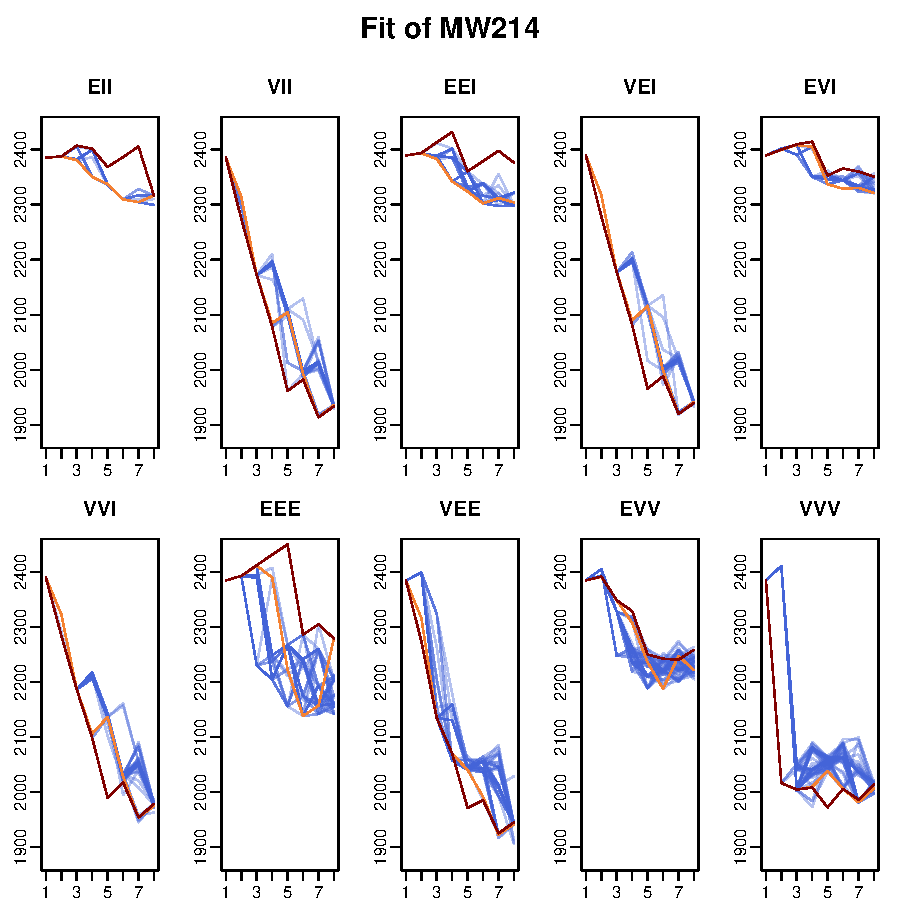
\includegraphics{chapter3-figMW214bic}
\end{figure}

here some examples of fitted mixtures

\begin{figure}
    \centering
\begin{Schunk}
\begin{Sinput}
>     f <- readRDS(file.path(savdir, claraMW[28]))
>     ff <- f$fit$nMm[8,8][[1]]
>     plot(ff$norMmix)
>     #points(ff$x)
\end{Sinput}
\end{Schunk}
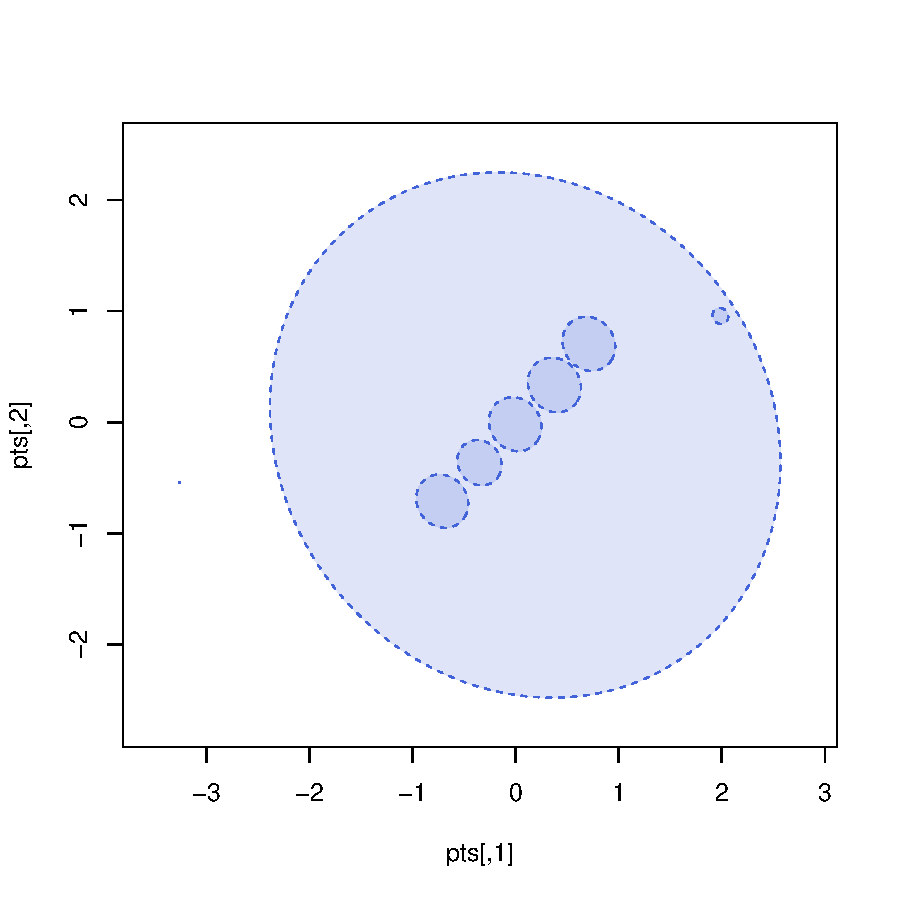
\includegraphics{chapter3-fig214fit}
\end{figure}

We can see, that, subtracting the obvious hiccups of the small erroneous
components, {\tt norMmix} has correctly found the 'intended' 
distribution. This is remarkable, given the small sample size and difficulty of distribution

\section{Nonnormal Mixtures}

here 2smi and 2var, maybe others as well.


here 2smi:

\begin{Schunk}
\begin{Sinput}
>     savdir <- file.path(mainsav, "2smi")
>     filenames <- list.files(savdir, pattern=".rds")
>     fnclara <- grep("clara_seed", filenames, value=TRUE)
>     fnmclVV <- grep("mclVVV_see", filenames, value=TRUE)
>     fnmclus <- grep("__mcl.rds",  filenames, value=TRUE)
\end{Sinput}
\end{Schunk}

\begin{figure}[h]
    \centering
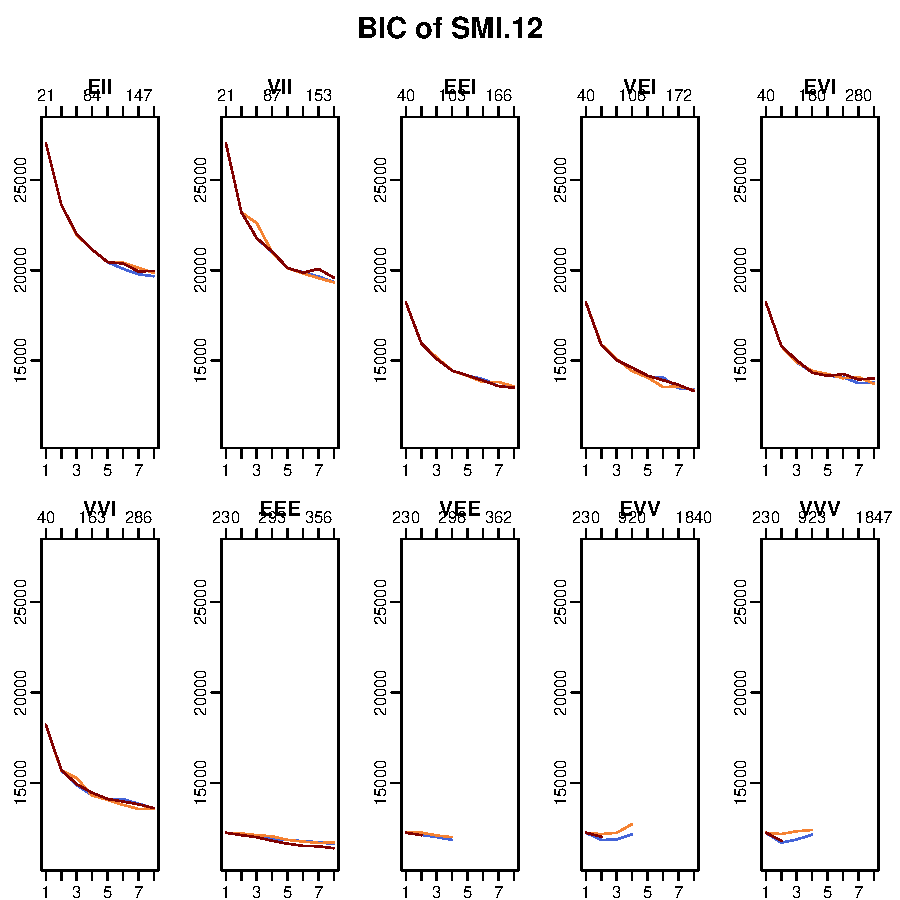
\includegraphics{chapter3-2smiplot}
\end{figure}

While not very spectacular, the graphs show that even at large parameter
counts our algorithm closes in on the same values as {\tt mclust}.
At these dimensions it is difficult to compare if these are actually 
equal, or even similar fits, but going by BIC values, it is at the very 
least equally viable as a working model.

To illustrate, here are the parameter sizes for this simulation:
\begin{Schunk}
\begin{Soutput}
  EII VII EEI VEI EVI VVI EEE VEE  EVV  VVV
1  21  21  40  40  40  40 230 230  230  230
2  42  43  61  62  80  81 251 252  460  461
3  63  65  82  84 120 122 272 274  690  692
4  84  87 103 106 160 163 293 296  920  923
5 105 109 124 128 200 204 314 318 1150 1154
6 126 131 145 150 240 245 335 340 1380 1385
7 147 153 166 172 280 286 356 362 1610 1616
8 168 175 187 194 320 327 377 384 1840 1847
\end{Soutput}
\end{Schunk}


